% Figures inductives finales. Dans ces figures, scRAW = trial0017.

\begin{figure}[htbp]
  \centering
  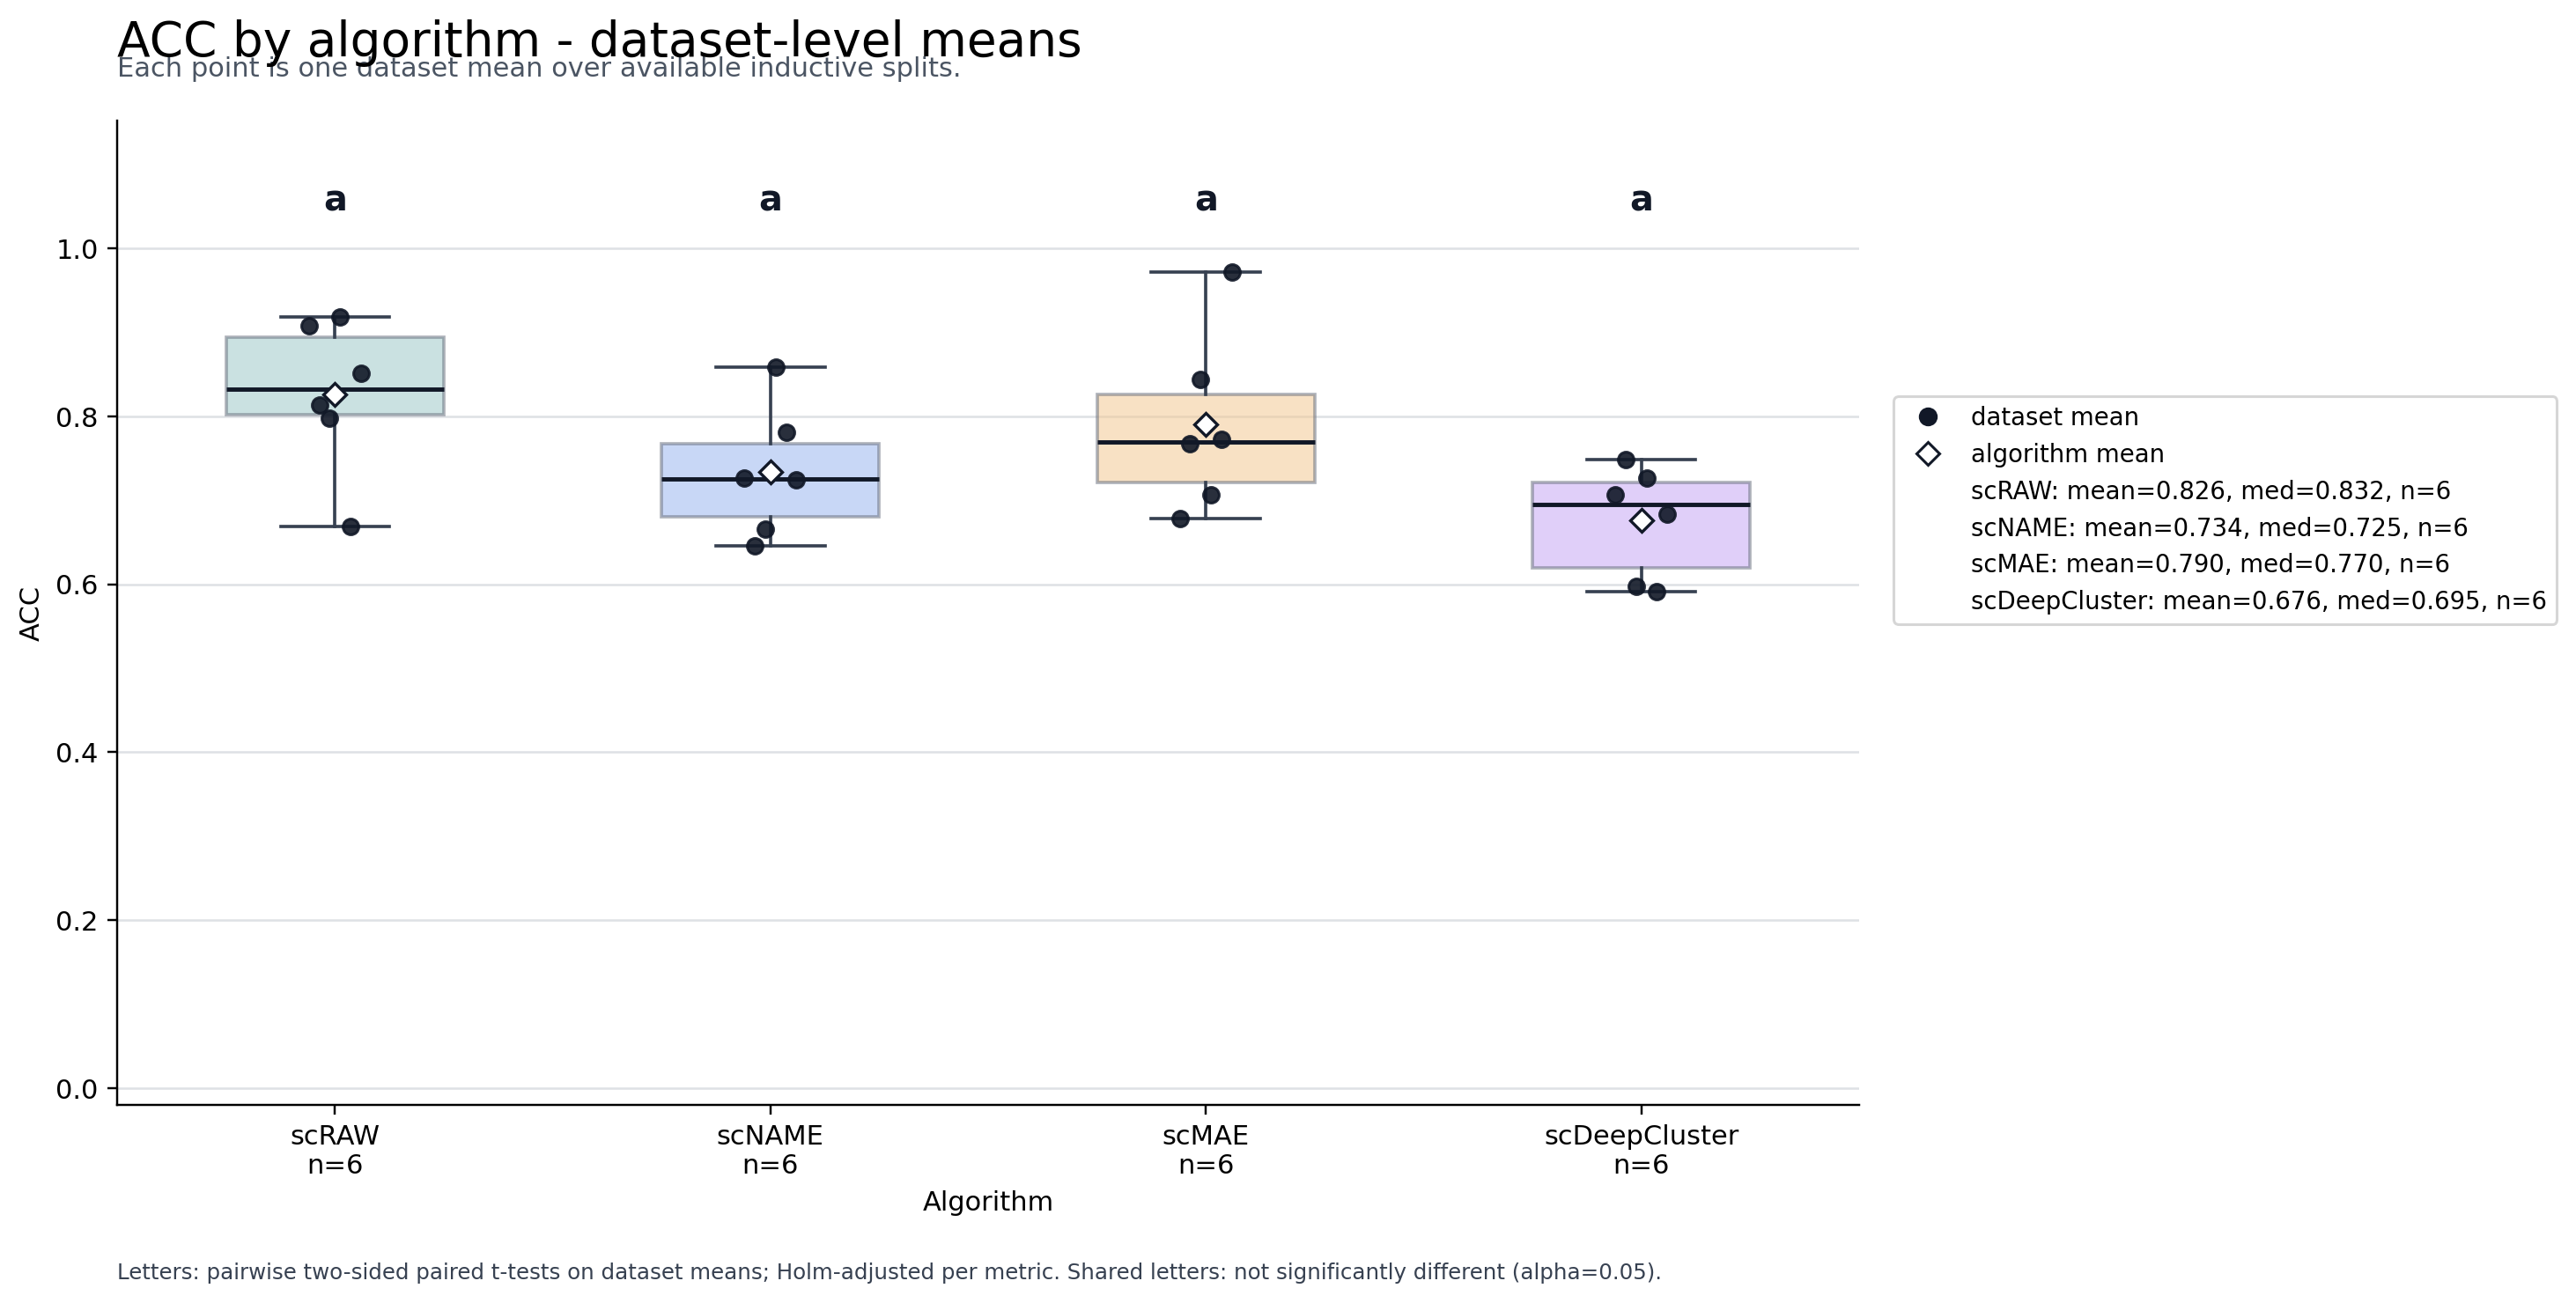
\includegraphics[width=0.95\linewidth]{Images/comparaison_inductive_scraw_trial0017_finale/ACC_by_algorithm_boxplot.png}
  \caption{Comparaison inductive des algorithmes selon l'ACC. Les points scRAW correspondent a la configuration trial0017.}
  \label{fig:inductive-acc-trial0017}
\end{figure}

\begin{figure}[htbp]
  \centering
  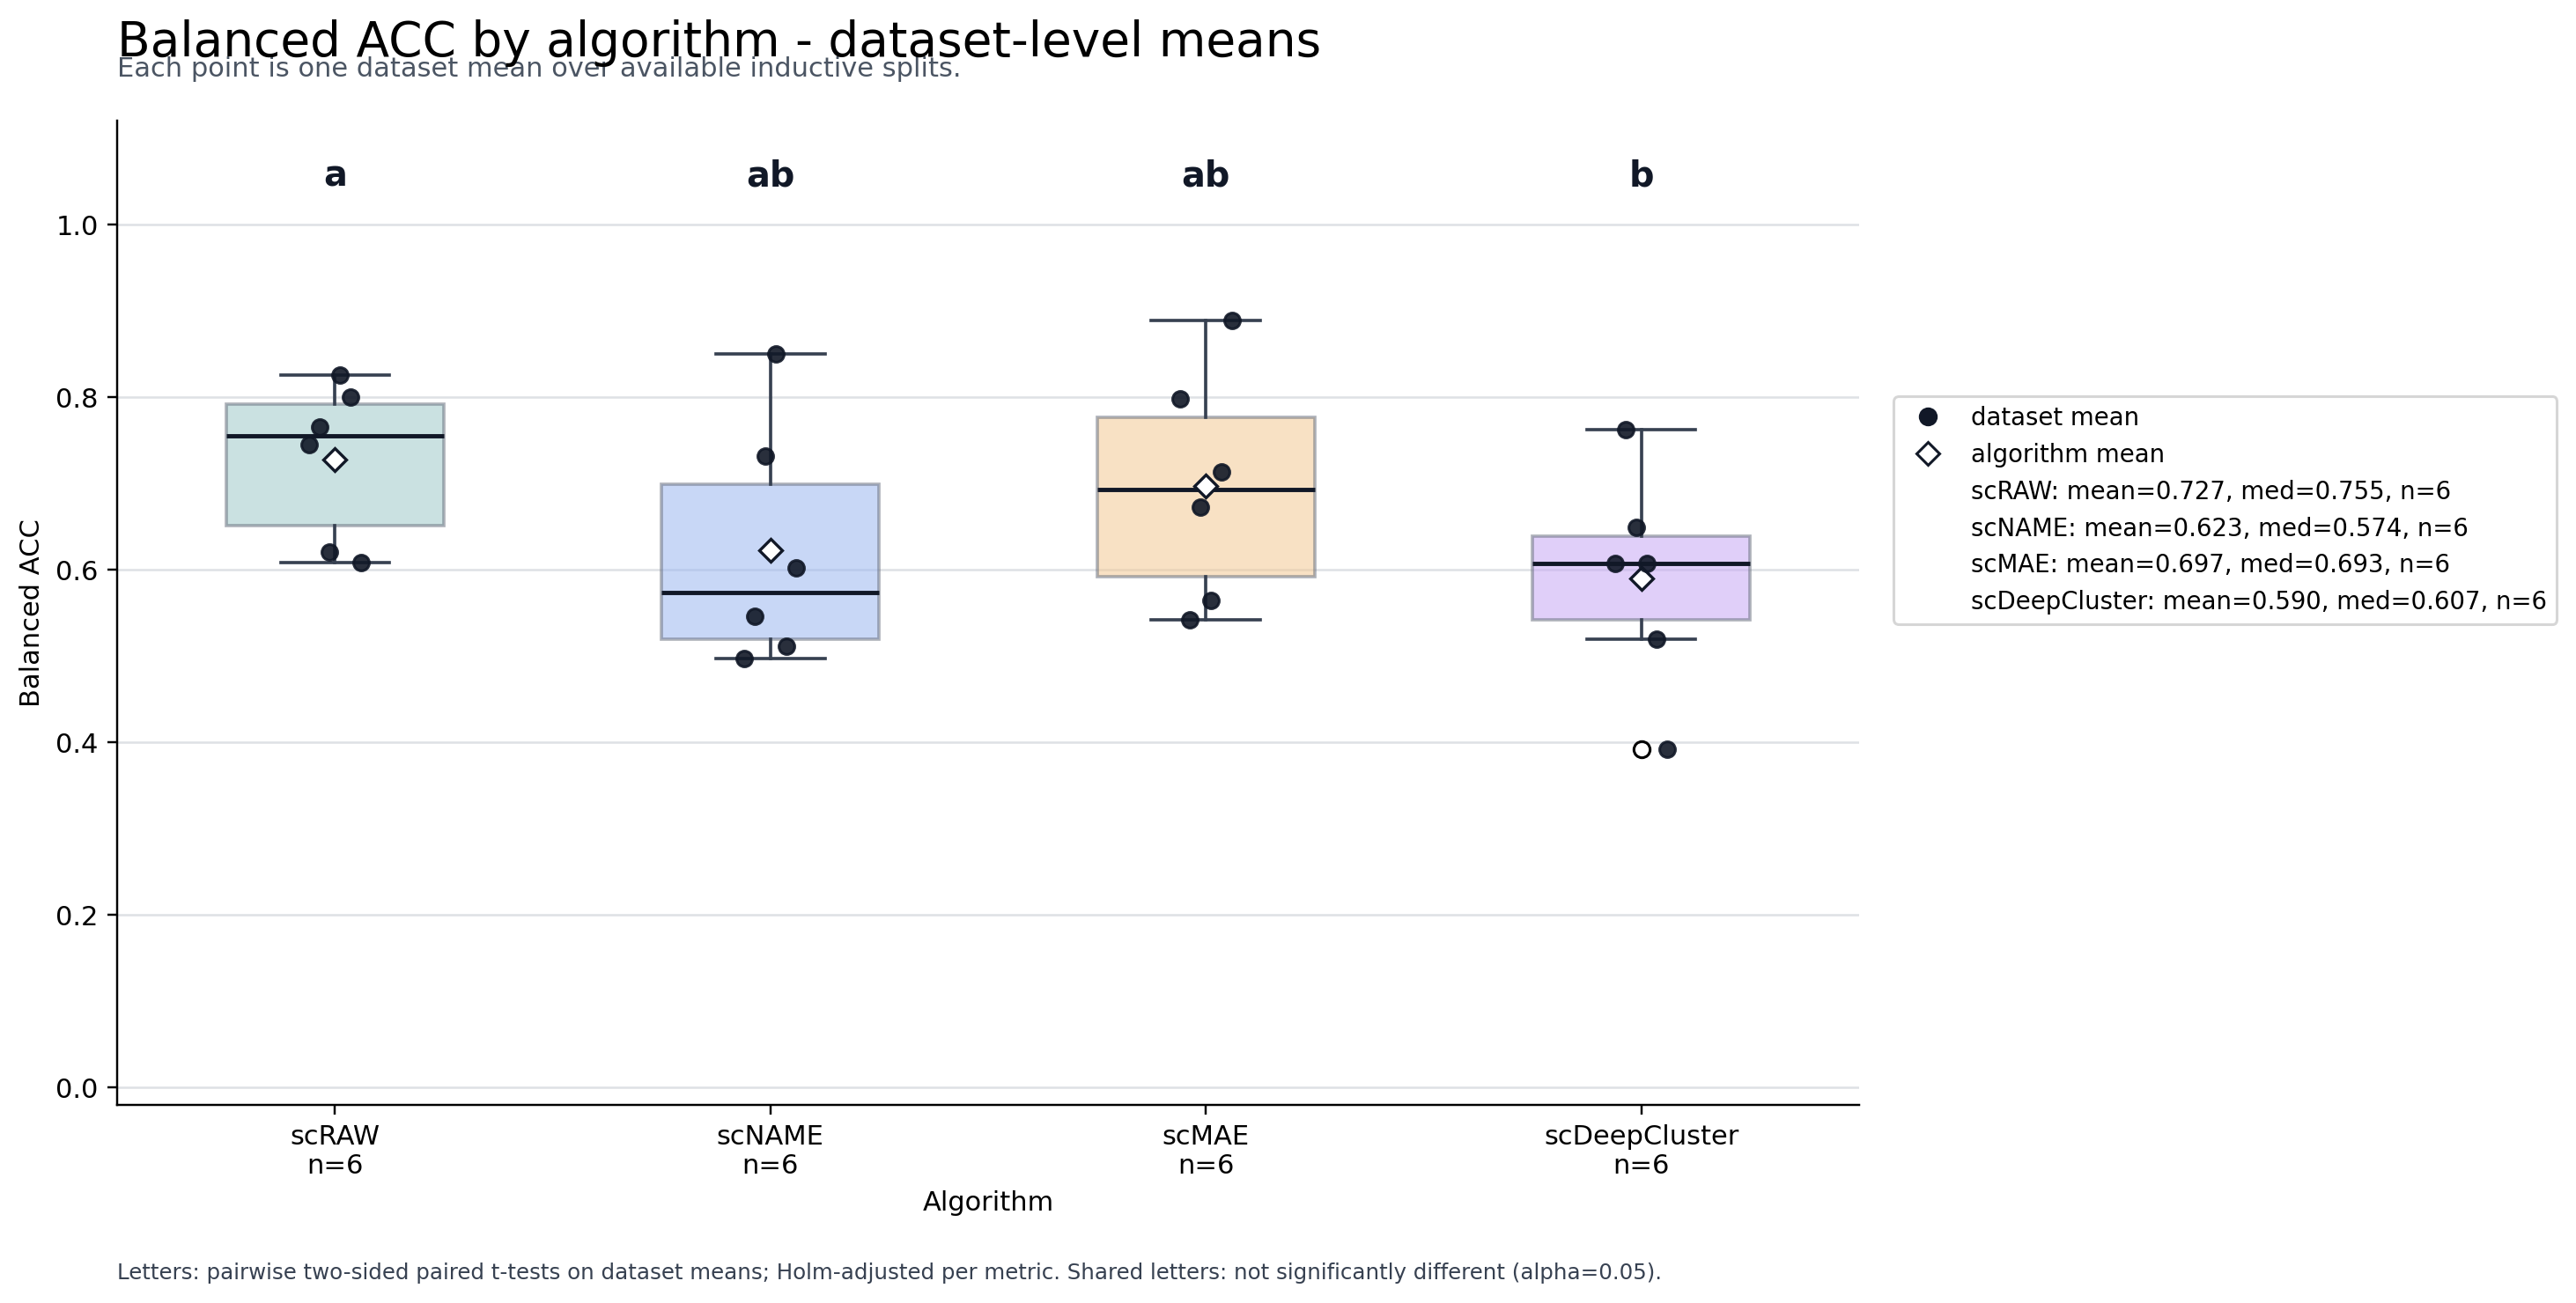
\includegraphics[width=0.95\linewidth]{Images/comparaison_inductive_scraw_trial0017_finale/BalancedACC_by_algorithm_boxplot.png}
  \caption{Comparaison inductive des algorithmes selon la Balanced Accuracy. Les points scRAW correspondent a la configuration trial0017.}
  \label{fig:inductive-balancedacc-trial0017}
\end{figure}

\begin{figure}[htbp]
  \centering
  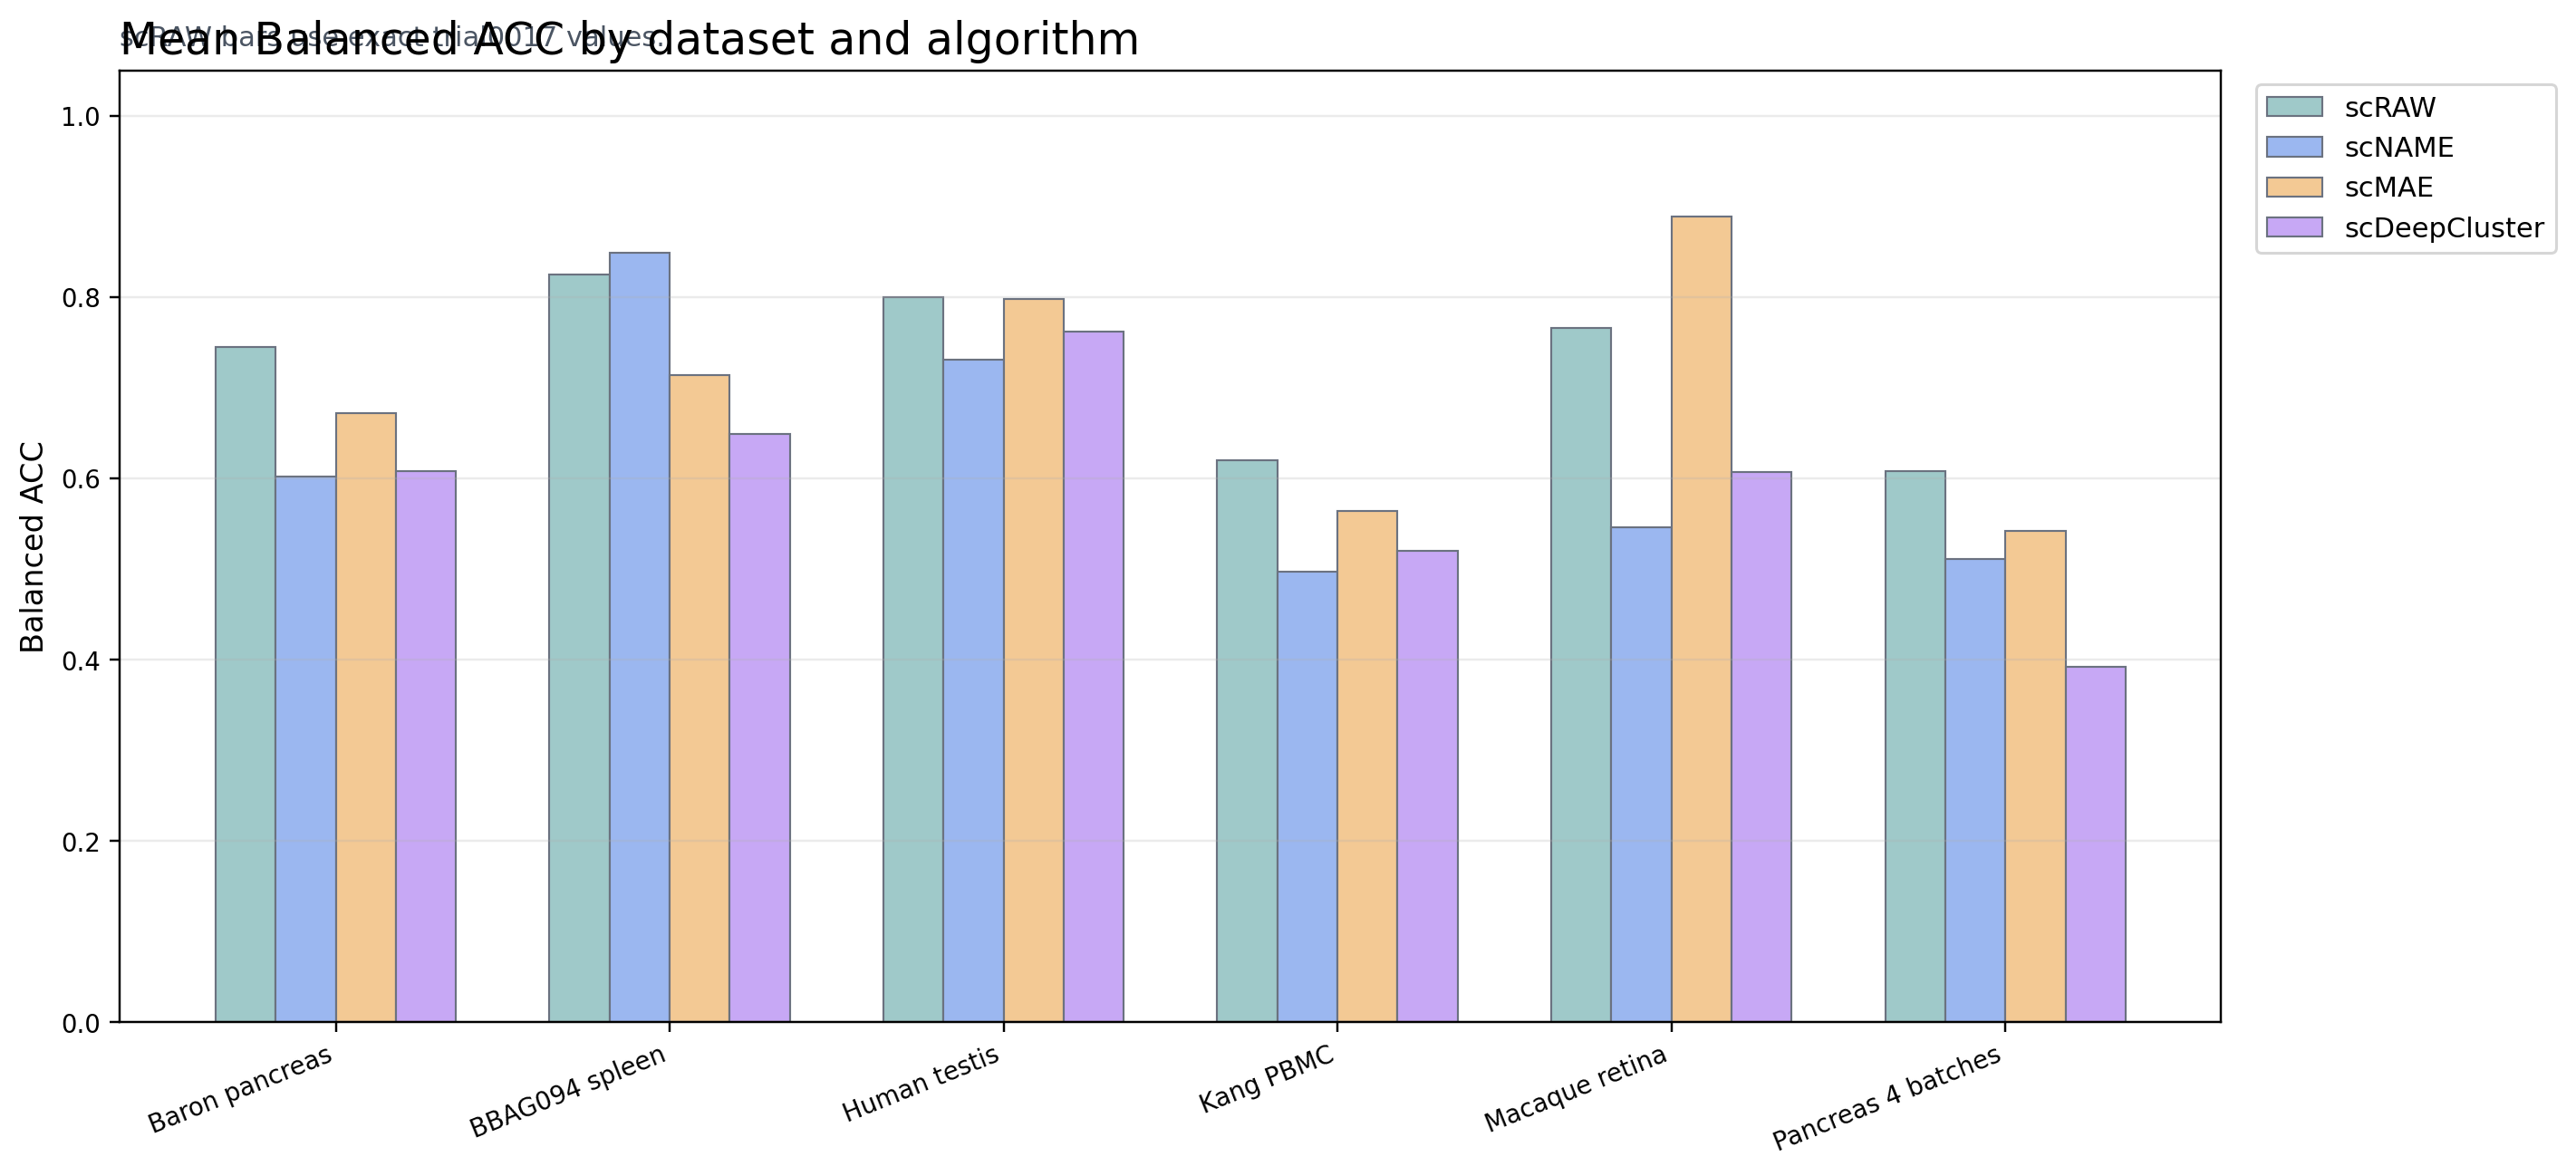
\includegraphics[width=0.95\linewidth]{Images/comparaison_inductive_scraw_trial0017_finale/mean_BalancedACC_by_dataset_algorithm.png}
  \caption{Balanced Accuracy moyenne par dataset et par algorithme en evaluation inductive. Les barres scRAW correspondent a la configuration trial0017.}
  \label{fig:inductive-balancedacc-datasets-trial0017}
\end{figure}

\begin{figure}[htbp]
  \centering
  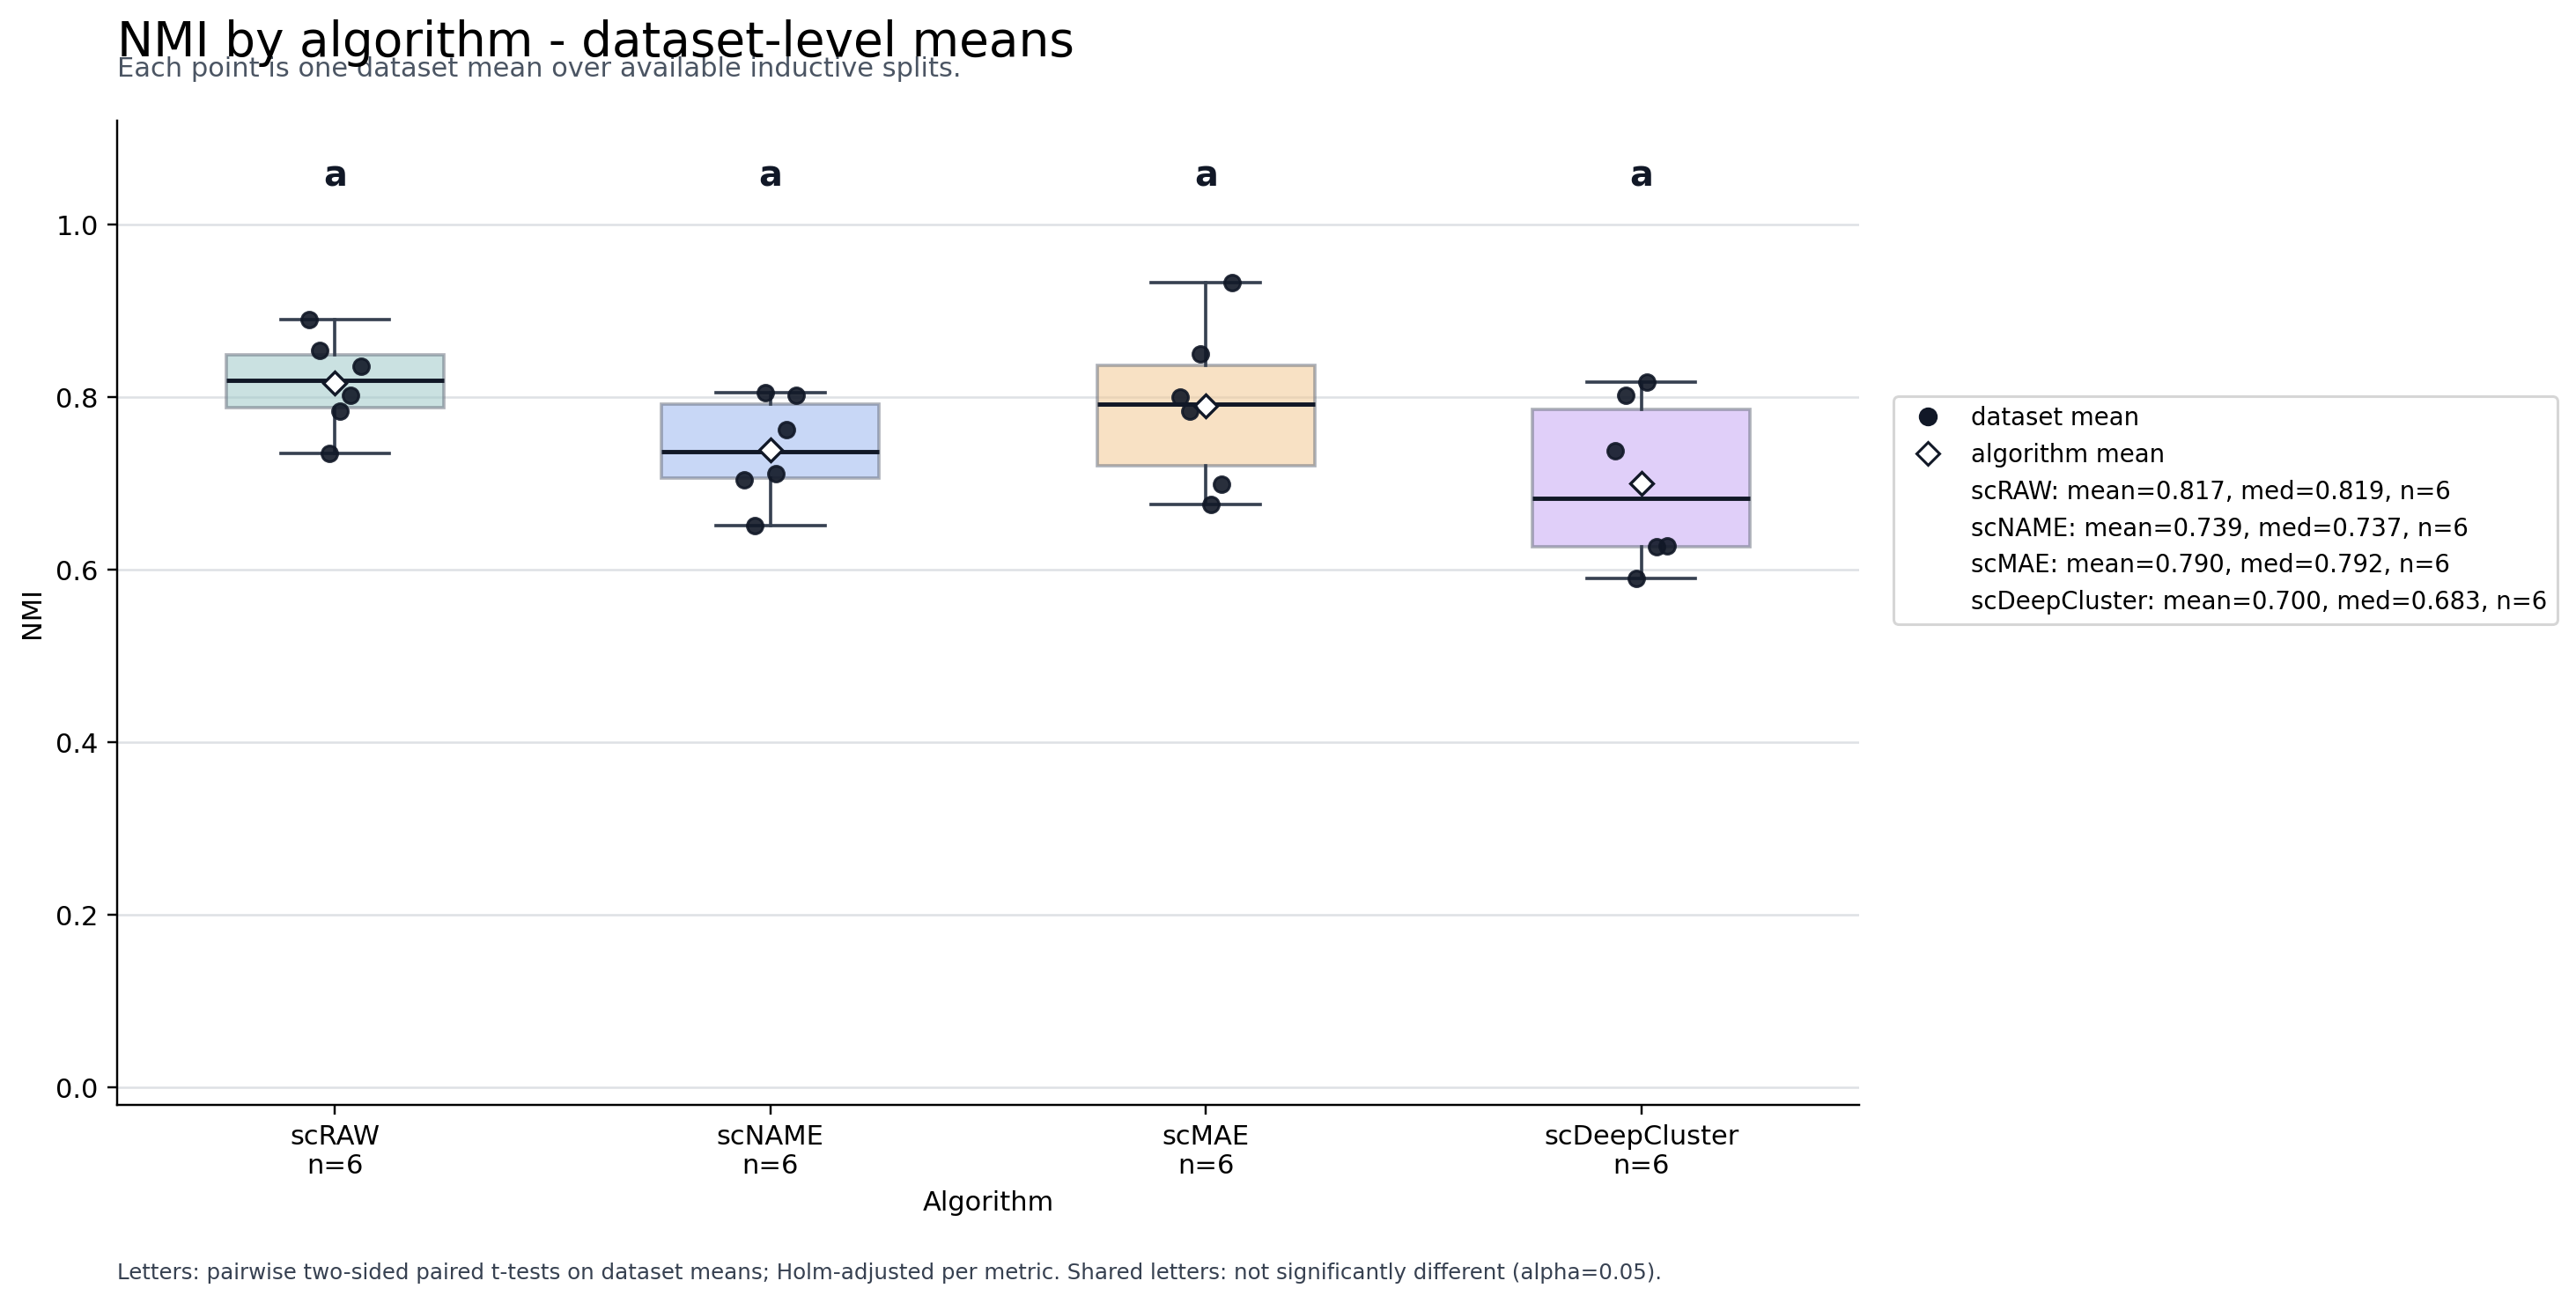
\includegraphics[width=0.95\linewidth]{Images/comparaison_inductive_scraw_trial0017_finale/NMI_by_algorithm_boxplot.png}
  \caption{Comparaison inductive des algorithmes selon la NMI. Les points scRAW correspondent a la configuration trial0017.}
  \label{fig:inductive-nmi-trial0017}
\end{figure}
